\documentclass[a4paper,11pt]{article}
\input{/home/tof/Documents/Cozy/latex-include/preambule_lua.tex}
\newcommand{\showprof}{show them}  % comment this line if you don't want to see todo environment
\fancyhead[L]{Exercices graphes - parcours}
\newdate{madate}{10}{09}{2020}
%\fancyhead[R]{\displaydate{madate}} %\today
%\fancyhead[R]{Seconde - SNT}
%\fancyhead[R]{Première - NSI}
\fancyhead[R]{Terminale - NSI}
\fancyfoot[L]{~\\Christophe Viroulaud}
\AtEndDocument{\label{lastpage}}
\fancyfoot[C]{\textbf{Page \thepage/\pageref{lastpage}}}
\fancyfoot[R]{\includegraphics[width=2cm,align=t]{/home/tof/Documents/Cozy/latex-include/cc.png}}
\usepackage{tikz}
\begin{document}
\begin{Form}
\begin{exo}
\begin{center}
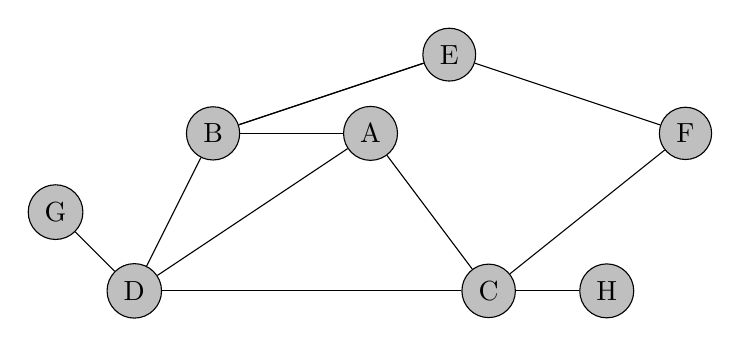
\begin{tikzpicture}
\node[draw,circle,fill=gray!50] (A)at(0,2) {A};
\node[draw,circle,fill=gray!50] (B)at(-2,2) {B};
\node[draw,circle,fill=gray!50] (C)at(1.5,0) {C};
\node[draw,circle,fill=gray!50] (D)at(-3,0) {D};
\node[draw,circle,fill=gray!50] (E)at(1,3) {E};
\node[draw,circle,fill=gray!50] (F)at(4,2) {F};
\node[draw,circle,fill=gray!50] (G)at(-4,1) {G};
\node[draw,circle,fill=gray!50] (H)at(3,0) {H};
\draw[-,>=latex] (A) -- (B);
\draw[-,>=latex] (A) -- (C);
\draw[-,>=latex] (A) -- (D);
\draw[-,>=latex] (D) -- (B);
\draw[-,>=latex] (B) -- (E);
\draw[-,>=latex] (B) -- (E);
\draw[-,>=latex] (D) -- (G);
\draw[-,>=latex] (C) -- (F);
\draw[-,>=latex] (C) -- (H);
\draw[-,>=latex] (C) -- (D);
\draw[-,>=latex] (E) -- (F);
\end{tikzpicture}
\captionof{figure}{Graphe à parcourir}
\label{graphe}
\end{center}
Pour les deux parcours il faudra détailler l'évolution de la structure utilisée (pile ou file) et le chemin final parcouru.
\begin{enumerate}
\item Quel est l'ordre du graphe \ref{graphe}?
\item Quel est le degré du sommet D?
\item Ce graphe est-il connexe?
\item Effectuer à la main un parcours en profondeur du graphe \ref{graphe}.
\item Effectuer à la main un parcours en largeur du graphe \ref{graphe}.
\end{enumerate}
\end{exo}
\begin{exo}
On souhaite organiser un tournoi entre 7 équipes de handball de telle manière que chaque équipe en rencontre 5 autres.
\begin{enumerate}
\item Une telle organisation est-elle possible? Justifier.
\item On désire maintenant que chaque équipe en rencontre quatre autres. Si cette organisation est possible, construire le graphe correspondant.
\end{enumerate}
\end{exo}
\begin{exo}
La ville de Königsberg (aujourd'hui Kaliningrad) est construite autour de deux îles situées sur le Pregel et reliées entre elles par un pont.
\begin{figure}[!h]
\centering
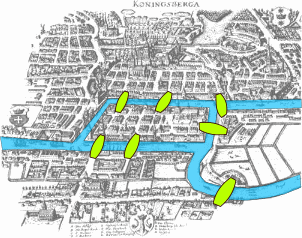
\includegraphics[width=5cm]{ressources/pont-konisberg.png}
\captionof{figure}{Les sept ponts de Königsberg}
\label{pont}
\end{figure}

Le problème, énoncé et résolu par Euler au XVIII° siècle, consiste à déterminer s'il existe une promenade permettant en partant d'un point, de revenir à ce même point en ayant traversé une et une seule fois chaque pont.
\begin{enumerate}
\item Modéliser la situation par un graphe.
\item Tenter de réaliser la promenade \guill{à la main}.
\end{enumerate}
Ce problème est à l'origine de \emph{la théorie des graphes}. C'est donc Euler qui commença à théoriser des problèmes mathématiques par cette méthode. Un vocabulaire spécifique a été crée en hommage.
\begin{center}
\shadowbox{\parbox{17cm}{\textbf{Définition:}
\begin{itemize}
\item une chaîne eulérienne est une chaîne passant une et une seule fois par toutes les arêtes du graphe.
\item un cycle eulérien est une chaîne eulérienne dont le sommet de départ et le sommet d'arrivée sont identiques. 
\end{itemize} 
\textbf{Théorème:}
\begin{itemize}
\item Un graphe connexe possède \textbf{une chaîne eulérienne} si et seulement si ses sommets sont tous de degré pair sauf au plus deux.
\item Un graphe connexe possède \textbf{un cycle eulérien} si et seulement si tous ses sommets sont de degré pair. 
\end{itemize}}}
\end{center}
\begin{enumerate}[resume]
\item Vérifier si le théorème est vérifié dans le cas des pont de Königsberg.
\item Peut-on créer une chaîne eulérienne pour le graphe \ref{graphe}? Et un cycle eulérien?
\end{enumerate}
\end{exo}
\begin{exo}
Le fonctionnement du parcours en profondeur peut être décrit de la manière suivante:
\begin{itemize}
\item Choisir un nœud.
\item S'il n'est pas déjà visité:
\begin{itemize}
\item le marquer \emph{vu},
\item pour chaque voisin, effectuer la même démarche.
\end{itemize}
\end{itemize}
Nous reconnaissons ici une démarche récursive.
\begin{enumerate}
\item Écrire la fonction \textbf{DFS\_rec(graphe: Graphe, sommet: str, visites: list=list())$\;\rightarrow\;$list} qui renvoie la liste des nœuds atteignables depuis \emph{sommet}. Nous utiliserons la classe \emph{Graphe} du cours (sans faire appel aux méthodes de parcours déjà élaborées).
\item Tester la fonction sur le graphe \ref{graphe}.
\item Comparer l'efficacité de cette fonction avec la méthode \emph{DFS} implémentée dans le cours.
\item Écrire alors la fonction \textbf{est\_connexe(graphe: Graphe)$\;\rightarrow\;$bool} qui renvoie \emph{True} si le graphe est connexe.
\item Écrire la fonction \textbf{DFS\_rec\_dico(graphe: Graphe, sommet: str, origine: str = None, visites: dict=\{\})$\;\rightarrow\;$dict} qui renvoie un dictionnaire des nœuds atteignables depuis \emph{sommet}. Le dictionnaire associera chaque sommet à son origine (sommet depuis lequel on l'a atteint).
\item Écrire la fonction \textbf{chemin(graphe: Graphe, depart: str, arrivee: str)$\;\rightarrow\;$list} qui renvoie un chemin entre \emph{depart} et \emph{arrivee}. Cette fonction utilisera \emph{DFS\_rec\_dico}. Il est à noter que le chemin obtenu n'est pas nécessairement le plus court.
\end{enumerate}
\begin{commentprof}
si on ne soucie pas de l'ordre on pourrait utiliser un ensemble (set). intérêt: coût mémoire, temps d'exécution\\
pour les + avancés: transformer les fonctions en méthodes dans Graphe
\end{commentprof}
\end{exo}
\begin{exo}
Il n'est pas obligatoire d'utiliser une file pour réaliser un parcours en largeur. Nous pouvons par exemple nous servir de deux ensembles:
\begin{itemize}
\item \textbf{voisins:} qui contiendra les sommets voisins du sommet d'origine,
\item \textbf{prochains:} qui contiendra les sommets à une distance $n+1$ du sommet d'origine et qui seront visités après ceux de l'ensemble \emph{voisins}.
\end{itemize}
Quand l'ensemble \emph{voisins} est vide, il suffit de le remplir avec les sommets de \emph{prochains}.
\begin{enumerate}
\item Écrire la fonction \textbf{BFS\_dico(graphe: Graphe, origine: str)$\;\rightarrow\;$dict} qui associe chaque sommet au sommet depuis lequel on l'a atteint lors du parcours en profondeur.
\item Écrire la fonction \textbf{chemin(graphe: Graphe, depart: str, arrivee: str)$\;\rightarrow\;$list} qui renvoie un chemin entre \emph{depart} et \emph{arrivee}. Cette fonction utilisera \emph{BFS\_dico}.
\end{enumerate}
\end{exo}
\end{Form}
\end{document}